\documentclass[xcolor=svgnames]{beamer}
\hypersetup{colorlinks,linkcolor=blue,urlcolor=blue}
\usetheme{Boadilla}

\usepackage[utf8]{inputenc}
\usepackage[T1]{fontenc}
\usepackage{lmodern}

\usepackage{listings}
\lstset{ %
  basicstyle=\footnotesize,
  breakatwhitespace=false,
  commentstyle=\color{DarkGreen}\ttfamily,
  frame=single,
  keepspaces=true,
  keywordstyle=\color{DarkBlue},
  language=Octave,
  morekeywords={*,...},
  numbers=none,
  showspaces=false,
  showstringspaces=false,
  showtabs=false,
  stringstyle=\color{DarkOrange},
  tabsize=2
}
\usepackage{mathtools}
\usepackage{tikz}
\usetikzlibrary{arrows,backgrounds,positioning,shadows,shapes}
\usetikzlibrary{decorations.pathreplacing}

\title{\texttt{publish} your code with Octave}
\author[Ohlhus]{Kai T. Ohlhus \\ \texttt{k.ohlhus@gmail.com}}
\institute{OctConf 2017}
\date{March 20, 2017}
\titlegraphic{
\vfill
\tiny
This work is licensed under a
Creative Commons Attribution-ShareAlike 4.0 International License.

\url{http://creativecommons.org/licenses/by-sa/4.0/}


\includegraphics[height=2em]{res/cc-by-sa.png}
}

\begin{document}

\frame{\titlepage}



\section{What is publish about?}



\subsection{1. Stale, outdated, incorrect example code.}



\begin{frame}[fragile]
\frametitle{What is \texttt{publish} about?}
\framesubtitle<2>{--- 1. Stale, outdated, incorrect example code.}

\begin{itemize}
\item Old \textsc{Matlab} teaching PDF
  with very simple example function {\color{blue}\lstinline|linear|}

\item Students trying to call their first function \underline{failed}!

\begin{lstlisting}[language={}]
>> y = linear(2)
Error using linear (line 52)
Invalid calling syntax for the "linear" command. Type
"help linear" for more information.
\end{lstlisting}

\item<2> The function \href{https://www.mathworks.com/help/ident/ref/linear.html}{linear}
became 2007 part of Matlab's System Identification Toolbox
\item<2> $\implies$ Need to rewrite documentation
\item<2> Decision to use \texttt{publish}
  (not part of GNU Octave before 4.2.0)
\end{itemize}
\end{frame}



\subsection{2. Display the output.}



\begin{frame}[fragile]
\frametitle{What is \texttt{publish} about?}
\framesubtitle{--- 2. Display the output.}

Most of Octave's example code is ``\textbf{static}'' as well:
\begin{itemize}
\item Copy \& run to see the output (\textit{incomplete?})
\item Never checked before a release (\textit{stale, outdated?})
\end{itemize}

\begin{lstlisting}[language={}]
>> help plot  # shortened

Here are some plot examples:

    t = 0:0.1:6.3;
    plot (t, cos(t), "-;cos(t);", t, sin(t), "-b;sin(t);");

This will plot the cosine and sine functions and label them
accordingly in the legend.
\end{lstlisting}

\begin{itemize}
\item Situation better with ``\texttt{doc plot}'' (or more descriptive Manual)
\end{itemize}

$\implies$ \textbf{Bad user experience, questions, bug reports}
{\tiny (\href{https://savannah.gnu.org/bugs/index.php?50282}{\#50282}
\href{https://savannah.gnu.org/bugs/index.php?50148}{\#50148},\ldots)}
\end{frame}


\subsection{3. Certainly no panacea!}


\begin{frame}
\frametitle{What is \texttt{publish} about?}
\framesubtitle{--- 3. Certainly \underline{\textbf{no}} panacea!}

Intended for ``small to medium'' sized \textbf{scripts}:
\begin{itemize}\itemsep1em
\item One section level
\item Supports HTML and \LaTeX\ (PDF) output (but see later)
\item No cross references (but URLs)
\item No function \textit{docstring} or class documentation
\end{itemize}

\vfill

$\implies$ No substitute for \LaTeX\ or Texinfo
\end{frame}



\section{Two short demos}



\begin{frame}[fragile]
\frametitle{Two short demos}

\begin{itemize}
\item Simple markup in comment blocks
\item \textbf{Execution} of example code, print results
\end{itemize}

\lstinputlisting[language=Octave]{demo1/script.m}

\begin{tikzpicture}[overlay]
\tikzstyle{label} = [red, midway, right=5mm]
\tikzstyle{brace} =
  [decorate, decoration={brace, mirror, amplitude=6pt}, thick, color=red]

\draw[brace] (5.5,4.6) -- ++ (0,1.5) node [label] {Documentation with markup};
\draw[brace] (5.5,3.3) -- ++ (0,1.2) node [label] {Example code with output};
\draw[brace] (5.5,0.6) -- ++ (0,1.4)
  node [label] {Example code with plot output};
\end{tikzpicture}
\end{frame}



\section{The publish -- grabcode workflow}



\begin{frame}
\frametitle{The \texttt{publish} -- \texttt{grabcode} workflow}

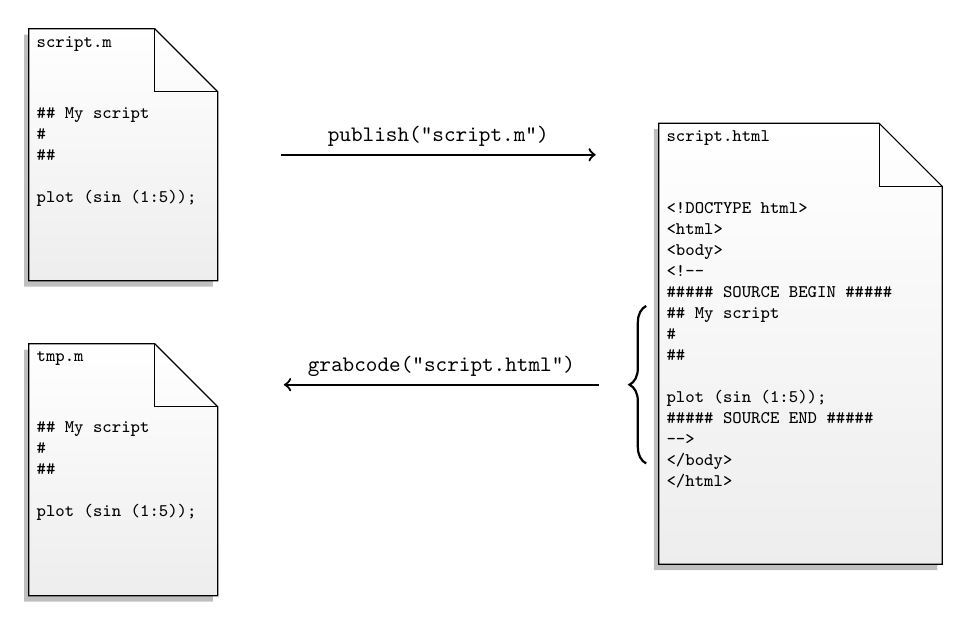
\begin{tikzpicture}[scale=0.8, every node/.style={scale=0.8}]
\tikzstyle{file} = [bottom color=black!7, top color=white,
  drop shadow={shadow xshift=-.4ex}]
\tikzstyle{content} = [align=left, font=\ttfamily\footnotesize]
\tikzstyle{brace} = [decorate, decoration={brace, mirror, amplitude=6pt}, thick]

\coordinate (script) at (0,0);
\draw[file] (script) -- ++(0,-4) -- ++(3,0)  -- ++(0,3) -- ++(-1,1) -- cycle;
\draw (script) ++(2,0) |- ++(1,-1);
\node[content,below right=0mm of script] { script.m \\[8mm]
  \#\# My script \\
  \# \\
  \#\# \\
  \\
  plot (sin (1:5)); \\
  };

\coordinate (tmp) at (0,-5);
\draw[file] (tmp) -- ++(0,-4) -- ++(3,0)  -- ++(0,3) -- ++(-1,1) -- cycle;
\draw (tmp) ++(2,0) |- ++(1,-1);
\node[content,below right=0mm of tmp] { tmp.m \\[8mm]
  \#\# My script \\
  \#\\
  \#\# \\
  \\
  plot (sin (1:5)); \\
  };

\coordinate (html) at (10,-1.5);
\draw[file] (html) -- ++(0,-7) -- ++(4.5,0)  -- ++(0,6) -- ++(-1,1) -- cycle;
\draw (html) ++(3.5,0) |- ++(1,-1);
\node[content,below right=0mm of html] { script.html \\[8mm]
  <!DOCTYPE html> \\
  <html> \\
  <body> \\
  <!-{-} \\
  \#\#\#\#\# SOURCE BEGIN \#\#\#\#\# \\
  \#\# My script \\
  \# \\
  \#\# \\
  \\
  plot (sin (1:5)); \\
  \#\#\#\#\# SOURCE END \#\#\#\#\# \\
  {-}-> \\
  </body> \\
  </html> \\
  };

\draw[->,thick] (script) ++ (4,-2) -- ++(5,0)
  node[midway, above] {\texttt{publish("script.m")}};
\draw [brace] (html) ++ (-0.2,-2.9) -- ++ (0,-2.5)
  coordinate [midway,left=0.6cm] (lbrace);
\draw[->,thick] (lbrace) -- ++(-5,0)
  node[midway, above] {\texttt{grabcode("script.html")}};
\end{tikzpicture}
\end{frame}



\section{Customize publish}



\begin{frame}
\frametitle{Customize \texttt{publish} (GNU Octave 4.3.0+)}

\begin{itemize}
\item Pure Octave code $\rightarrow$ easy to extend/modify
\item Designed for extension:
  \begin{itemize}
  \item Implement all callback subfunctions in some
    {\color{blue}\lstinline|__publish_my_markup_output__.m|} and run
    \lstinline|publish("script.m", "my_markup")|
  \end{itemize}
\item Some interesting experiment with MediaWiki action API\footnote{Read more: \url{https://siko1056.github.io/blog/2017/03/10/getting-to-know-the-mediawiki-api.html}.}.
\end{itemize}

\begin{center}
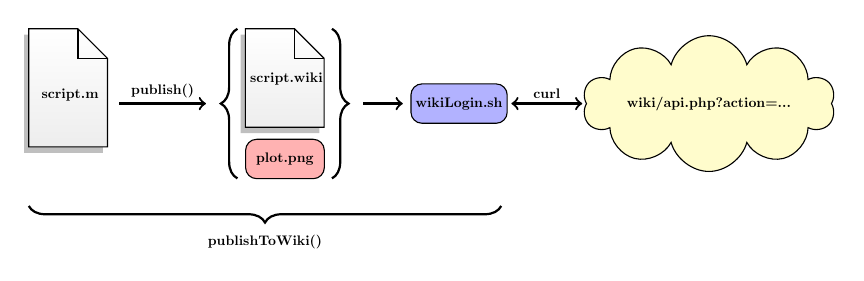
\begin{tikzpicture}[scale=0.5, every node/.style={scale=0.5}]
\tikzstyle{box} = [rectangle, rounded corners, minimum width=2cm,
  minimum height=1cm, text centered, draw=black]
\tikzstyle{brace} = [decorate, decoration={brace, amplitude=6pt}, thick]
\tikzstyle{file} = [bottom color=black!7, top color=white,
  drop shadow={shadow xshift=-.4ex}]
\tikzstyle{wikicloud} = [cloud, draw=black, fill=yellow!20, aspect=3]

\coordinate (script) at (0,0);
\draw[file] (script) -- ++(0,-3) -- ++(2,0)  -- ++(0,2.25) -- ++(-0.75,0.75)
                     -- cycle;
\draw (script) ++(1.25,0) |- ++(0.75,-0.75);
\node[align=left,below right=7mm and 1mm of script] {\textbf{script.m}};

\coordinate (scriptwiki) at (5.5,0);
\draw[file] (scriptwiki) -- ++(0,-2.5) -- ++(2,0)  -- ++(0,1.75)
                         -- ++(-0.75,0.75) -- cycle;
\draw (scriptwiki) ++(1.25,0) |- ++(0.75,-0.75);
\node[align=left,below right=5mm and 0mm of scriptwiki] {\textbf{script.wiki}};

\node[box, fill=red!30, below right=14mm and 0mm of scriptwiki]
  {\textbf{plot.png}};

\draw[brace] (scriptwiki) ++ (-0.2,-3.8) -- ++ (0,3.8)
  coordinate[midway] (lbrace);
\draw[brace] (scriptwiki) ++ (2.2,0) -- ++ (0,-3.8) coordinate[midway] (rbrace);

\draw[<-,thick] (lbrace) ++ (-0.8,0) -- ++(-2.2,0)
  node[midway, above] {\textbf{publish()}};
\draw[->,thick] (rbrace) ++ (0.8,0) -- ++(1,0);

\node[box, fill=blue!30, right=of rbrace] (loginsh) {\textbf{wikiLogin.sh}};

\node[wikicloud, right=of loginsh] {\textbf{wiki/api.php?action=...}};

\draw[<->,thick] (loginsh.east) ++ (0.1,0) -- ++ (1.8,0)
  node[midway, above] {\textbf{curl}};

\draw[brace] (script) ++ (12,-4.5) -- ++ (-12,0)
  node[midway, below=3mm] {\textbf{publishToWiki()}};
\end{tikzpicture}
\end{center}
\end{frame}



\section{A new Agora approach?}



\begin{frame}
\frametitle{A new Agora approach?}
\framesubtitle{--- Maybe GSoC 2017 project?}

\begin{itemize}
\item Pros:
  \begin{itemize}
  \item Login system
  \item History (revert vandalism)
  \item Editor
  \item Syntax highlighting
  \end{itemize}
\item Cons:
  \begin{itemize}
  \item Expose \texttt{api.php} (\textit{security concern?})
  \item Image storage limitation
  \item Login required (\textit{limited access / vandalism})
  \item Deal with HTML escaping
  \end{itemize}
\item \texttt{urlread} cannot handle \textbf{session cookies}.
  The demo relies on \texttt{bash} script calling \texttt{curl}
  appropriately. $\rightarrow$ This can be fixed.
\end{itemize}
\end{frame}



\begin{frame}
\begin{center}
\Huge
Thank you for your attention.

Questions?

\vfill

\normalsize
Find the sources at \url{https://github.com/siko1056/OctConf2017}.
\end{center}
\end{frame}



\begin{frame}[noframenumbering]
\frametitle{Discussion: A survey of documentation}

\begin{itemize}
\item \href{http://hg.savannah.gnu.org/hgweb/octave/file/tip/doc}{Octave repo}
  (\href{https://savannah.gnu.org/project/memberlist.php?group=octave}{24}
  committers, overwhelming bug reports)
  \begin{itemize}
  \item \href{https://www.gnu.org/software/octave/doc/interpreter/}{Manual}
    for end-users, description, and function reference
    \begin{itemize}
    \item updated with each releases (~twice each year)
    \end{itemize}
  \item \href{http://wiki.octave.org/Doxygen}{Doxygen} (C/C++ only)
    \begin{itemize}
    \item not actively presented, not updated
    \end{itemize}
  \end{itemize}
\item \href{https://octave.sourceforge.io}{Octave forge}
  (\textit{~70} maintainers?)
  \begin{itemize}
  \item individual package docs, updates by maintainers
  \item Octave core and package
  \href{https://octave.sourceforge.io/octave/overview.html}{function reference}
  \end{itemize}
\item \href{http://wiki.octave.or}{Wiki}
  (\href{http://wiki.octave.org/Special:Statistics}{~25 active and ~600 passive})
  registered users)
  \begin{itemize}
  \item docs for installation, forge packages, contribution guidelines, ...
  \item updated occasionally, not release specific, many outdated articles
  \end{itemize}
\end{itemize}
\end{frame}



\begin{frame}[noframenumbering]
\frametitle{Discussion: A survey of documentation (cont.)}

\begin{itemize}
\item \textbf{Manual} (static, \textbf{dynamic} graphic generation)
  \begin{itemize}
  \item \href{https://www.gnu.org/software/texinfo/manual/texinfo/texinfo.html}{Texinfo}
    and helper scripts (AWK, Bash, Octave, Perl)
  \item HTML, PDF output
  \item markup, links
  \end{itemize}
\item \textbf{Doxygen} (static, \textbf{dynamic} completeness checking)
  \begin{itemize}
  \item Special
    \href{http://www.stack.nl/~dimitri/doxygen/manual/index.html}{comment blocks},
    no real overhead
  \item (very rich) HTML, LaTeX, RTF, XML, Man page, DocBook output
  \item markup (Markdown), links
  \end{itemize}
\item \textbf{Wiki} (static)
  \begin{itemize}
  \item the power of
    \href{https://www.mediawiki.org/wiki/Help:Formatting}{MediaWiki}
  \item not related to Octave (but syntax highlighting!)
  \end{itemize}
\item \textbf{Octave forge packages} (static, dynamic elements?)
  \begin{itemize}
  \item \href{https://www.gnu.org/software/texinfo/manual/texinfo/texinfo.html}{Texinfo}
  and \href{https://octave.sourceforge.io/generate_html}{generate\_html} package
  \item HTML
  \item markup, links
  \end{itemize}
\end{itemize}
\end{frame}

\end{document}